% Options for packages loaded elsewhere
\PassOptionsToPackage{unicode}{hyperref}
\PassOptionsToPackage{hyphens}{url}
\PassOptionsToPackage{dvipsnames,svgnames,x11names}{xcolor}
%
\documentclass[
  letterpaper,
  DIV=11,
  numbers=noendperiod]{scrartcl}

\usepackage{amsmath,amssymb}
\usepackage{iftex}
\ifPDFTeX
  \usepackage[T1]{fontenc}
  \usepackage[utf8]{inputenc}
  \usepackage{textcomp} % provide euro and other symbols
\else % if luatex or xetex
  \usepackage{unicode-math}
  \defaultfontfeatures{Scale=MatchLowercase}
  \defaultfontfeatures[\rmfamily]{Ligatures=TeX,Scale=1}
\fi
\usepackage{lmodern}
\ifPDFTeX\else  
    % xetex/luatex font selection
\fi
% Use upquote if available, for straight quotes in verbatim environments
\IfFileExists{upquote.sty}{\usepackage{upquote}}{}
\IfFileExists{microtype.sty}{% use microtype if available
  \usepackage[]{microtype}
  \UseMicrotypeSet[protrusion]{basicmath} % disable protrusion for tt fonts
}{}
\makeatletter
\@ifundefined{KOMAClassName}{% if non-KOMA class
  \IfFileExists{parskip.sty}{%
    \usepackage{parskip}
  }{% else
    \setlength{\parindent}{0pt}
    \setlength{\parskip}{6pt plus 2pt minus 1pt}}
}{% if KOMA class
  \KOMAoptions{parskip=half}}
\makeatother
\usepackage{xcolor}
\setlength{\emergencystretch}{3em} % prevent overfull lines
\setcounter{secnumdepth}{-\maxdimen} % remove section numbering
% Make \paragraph and \subparagraph free-standing
\makeatletter
\ifx\paragraph\undefined\else
  \let\oldparagraph\paragraph
  \renewcommand{\paragraph}{
    \@ifstar
      \xxxParagraphStar
      \xxxParagraphNoStar
  }
  \newcommand{\xxxParagraphStar}[1]{\oldparagraph*{#1}\mbox{}}
  \newcommand{\xxxParagraphNoStar}[1]{\oldparagraph{#1}\mbox{}}
\fi
\ifx\subparagraph\undefined\else
  \let\oldsubparagraph\subparagraph
  \renewcommand{\subparagraph}{
    \@ifstar
      \xxxSubParagraphStar
      \xxxSubParagraphNoStar
  }
  \newcommand{\xxxSubParagraphStar}[1]{\oldsubparagraph*{#1}\mbox{}}
  \newcommand{\xxxSubParagraphNoStar}[1]{\oldsubparagraph{#1}\mbox{}}
\fi
\makeatother

\usepackage{color}
\usepackage{fancyvrb}
\newcommand{\VerbBar}{|}
\newcommand{\VERB}{\Verb[commandchars=\\\{\}]}
\DefineVerbatimEnvironment{Highlighting}{Verbatim}{commandchars=\\\{\}}
% Add ',fontsize=\small' for more characters per line
\usepackage{framed}
\definecolor{shadecolor}{RGB}{241,243,245}
\newenvironment{Shaded}{\begin{snugshade}}{\end{snugshade}}
\newcommand{\AlertTok}[1]{\textcolor[rgb]{0.68,0.00,0.00}{#1}}
\newcommand{\AnnotationTok}[1]{\textcolor[rgb]{0.37,0.37,0.37}{#1}}
\newcommand{\AttributeTok}[1]{\textcolor[rgb]{0.40,0.45,0.13}{#1}}
\newcommand{\BaseNTok}[1]{\textcolor[rgb]{0.68,0.00,0.00}{#1}}
\newcommand{\BuiltInTok}[1]{\textcolor[rgb]{0.00,0.23,0.31}{#1}}
\newcommand{\CharTok}[1]{\textcolor[rgb]{0.13,0.47,0.30}{#1}}
\newcommand{\CommentTok}[1]{\textcolor[rgb]{0.37,0.37,0.37}{#1}}
\newcommand{\CommentVarTok}[1]{\textcolor[rgb]{0.37,0.37,0.37}{\textit{#1}}}
\newcommand{\ConstantTok}[1]{\textcolor[rgb]{0.56,0.35,0.01}{#1}}
\newcommand{\ControlFlowTok}[1]{\textcolor[rgb]{0.00,0.23,0.31}{\textbf{#1}}}
\newcommand{\DataTypeTok}[1]{\textcolor[rgb]{0.68,0.00,0.00}{#1}}
\newcommand{\DecValTok}[1]{\textcolor[rgb]{0.68,0.00,0.00}{#1}}
\newcommand{\DocumentationTok}[1]{\textcolor[rgb]{0.37,0.37,0.37}{\textit{#1}}}
\newcommand{\ErrorTok}[1]{\textcolor[rgb]{0.68,0.00,0.00}{#1}}
\newcommand{\ExtensionTok}[1]{\textcolor[rgb]{0.00,0.23,0.31}{#1}}
\newcommand{\FloatTok}[1]{\textcolor[rgb]{0.68,0.00,0.00}{#1}}
\newcommand{\FunctionTok}[1]{\textcolor[rgb]{0.28,0.35,0.67}{#1}}
\newcommand{\ImportTok}[1]{\textcolor[rgb]{0.00,0.46,0.62}{#1}}
\newcommand{\InformationTok}[1]{\textcolor[rgb]{0.37,0.37,0.37}{#1}}
\newcommand{\KeywordTok}[1]{\textcolor[rgb]{0.00,0.23,0.31}{\textbf{#1}}}
\newcommand{\NormalTok}[1]{\textcolor[rgb]{0.00,0.23,0.31}{#1}}
\newcommand{\OperatorTok}[1]{\textcolor[rgb]{0.37,0.37,0.37}{#1}}
\newcommand{\OtherTok}[1]{\textcolor[rgb]{0.00,0.23,0.31}{#1}}
\newcommand{\PreprocessorTok}[1]{\textcolor[rgb]{0.68,0.00,0.00}{#1}}
\newcommand{\RegionMarkerTok}[1]{\textcolor[rgb]{0.00,0.23,0.31}{#1}}
\newcommand{\SpecialCharTok}[1]{\textcolor[rgb]{0.37,0.37,0.37}{#1}}
\newcommand{\SpecialStringTok}[1]{\textcolor[rgb]{0.13,0.47,0.30}{#1}}
\newcommand{\StringTok}[1]{\textcolor[rgb]{0.13,0.47,0.30}{#1}}
\newcommand{\VariableTok}[1]{\textcolor[rgb]{0.07,0.07,0.07}{#1}}
\newcommand{\VerbatimStringTok}[1]{\textcolor[rgb]{0.13,0.47,0.30}{#1}}
\newcommand{\WarningTok}[1]{\textcolor[rgb]{0.37,0.37,0.37}{\textit{#1}}}

\providecommand{\tightlist}{%
  \setlength{\itemsep}{0pt}\setlength{\parskip}{0pt}}\usepackage{longtable,booktabs,array}
\usepackage{calc} % for calculating minipage widths
% Correct order of tables after \paragraph or \subparagraph
\usepackage{etoolbox}
\makeatletter
\patchcmd\longtable{\par}{\if@noskipsec\mbox{}\fi\par}{}{}
\makeatother
% Allow footnotes in longtable head/foot
\IfFileExists{footnotehyper.sty}{\usepackage{footnotehyper}}{\usepackage{footnote}}
\makesavenoteenv{longtable}
\usepackage{graphicx}
\makeatletter
\def\maxwidth{\ifdim\Gin@nat@width>\linewidth\linewidth\else\Gin@nat@width\fi}
\def\maxheight{\ifdim\Gin@nat@height>\textheight\textheight\else\Gin@nat@height\fi}
\makeatother
% Scale images if necessary, so that they will not overflow the page
% margins by default, and it is still possible to overwrite the defaults
% using explicit options in \includegraphics[width, height, ...]{}
\setkeys{Gin}{width=\maxwidth,height=\maxheight,keepaspectratio}
% Set default figure placement to htbp
\makeatletter
\def\fps@figure{htbp}
\makeatother

\KOMAoption{captions}{tableheading}
\makeatletter
\@ifpackageloaded{caption}{}{\usepackage{caption}}
\AtBeginDocument{%
\ifdefined\contentsname
  \renewcommand*\contentsname{Table of contents}
\else
  \newcommand\contentsname{Table of contents}
\fi
\ifdefined\listfigurename
  \renewcommand*\listfigurename{List of Figures}
\else
  \newcommand\listfigurename{List of Figures}
\fi
\ifdefined\listtablename
  \renewcommand*\listtablename{List of Tables}
\else
  \newcommand\listtablename{List of Tables}
\fi
\ifdefined\figurename
  \renewcommand*\figurename{Figure}
\else
  \newcommand\figurename{Figure}
\fi
\ifdefined\tablename
  \renewcommand*\tablename{Table}
\else
  \newcommand\tablename{Table}
\fi
}
\@ifpackageloaded{float}{}{\usepackage{float}}
\floatstyle{ruled}
\@ifundefined{c@chapter}{\newfloat{codelisting}{h}{lop}}{\newfloat{codelisting}{h}{lop}[chapter]}
\floatname{codelisting}{Listing}
\newcommand*\listoflistings{\listof{codelisting}{List of Listings}}
\makeatother
\makeatletter
\makeatother
\makeatletter
\@ifpackageloaded{caption}{}{\usepackage{caption}}
\@ifpackageloaded{subcaption}{}{\usepackage{subcaption}}
\makeatother

\ifLuaTeX
  \usepackage{selnolig}  % disable illegal ligatures
\fi
\usepackage{bookmark}

\IfFileExists{xurl.sty}{\usepackage{xurl}}{} % add URL line breaks if available
\urlstyle{same} % disable monospaced font for URLs
\hypersetup{
  pdftitle={Supplementary Material},
  colorlinks=true,
  linkcolor={blue},
  filecolor={Maroon},
  citecolor={Blue},
  urlcolor={Blue},
  pdfcreator={LaTeX via pandoc}}


\title{Supplementary Material}
\author{}
\date{}

\begin{document}
\maketitle


\subsection{Multi-objective Optimization to Derive an SPI
target}\label{multi-objective-optimization-to-derive-an-spi-target}

To set up the optimisation task, we first need to express the parameter
space and any constraints. Since our goal is to identify an optimised
soundscape target distribution, the parameters we will search over are:

\begin{itemize}
\item
  \(\xi = (\xi_x, \xi_y)\), \(-1 \leq \xi \leq 1\)
\item
  \(\Omega = \begin{pmatrix} var(x) & cov(x, y) \\ cov(y, x) & var(y) \end{pmatrix}\)

  \begin{itemize}
  \tightlist
  \item
    \(0 \leq var() \leq 1\)
  \item
    \(-1 \leq cov() \leq 1\)
  \item
    \(\Omega\) must be symmetric and positive definite
  \end{itemize}
\item
  \(\alpha = (\alpha_x, \alpha_y)\), \(-5 \leq \alpha \leq 5\)
\item
  \(-1 \leq x, y \leq 1\) In \texttt{pymoo}, each objective function is
  supposed to be minimized. Therefore, we need to convert both SPI and
  r() to minimize problems.
\item
  min \(-r(ranks_{quality}, ranks_{target})\)
\item
  min \(-mean(SPI_{target}(X_i))\)
\end{itemize}

The final objective function is:

\begin{itemize}
\tightlist
\item
  \(f_1 = -r(ranks_{quality}, ranks_{target})\)
\item
  \(f_2 = -mean(SPI_{target}(X_i))\)
\end{itemize}

So our variables to optimize are:

\begin{itemize}
\tightlist
\item
  \(-1 \leq \xi_x \leq 1\)
\item
  \(-1 \leq \xi_y \leq 1\)
\item
  \(0 \leq var(x) \leq 1\)
\item
  \(0 \leq var(y) \leq 1\)
\item
  \(-1 \leq cov(x, y) \leq 1\)
\item
  \(-5 \leq \alpha_x \leq 5\)
\item
  \(-5 \leq \alpha_y \leq 5\)
\end{itemize}

Constraint: - \(\Omega\) must be symmetric and positive definite -
\texttt{np.linalg.eigvals(omega)\ \textgreater{}\ 0}

We then define the objective functions based on the two goals given
above. For each step in the algorithm with a given trial set of
parameters, a target distribution will be produced, the SPI for each
test location assessed according to the protocol described in
Section\textasciitilde{}\ref{sec-method}, and the resulting set of SPI
scores and ranking will be scored using the objective functions. Goal
(1) is assessed by calculating the Spearman rank correlation between the
\emph{a priori} ranking and the SPI ranking:

\begin{Shaded}
\begin{Highlighting}[]
\ImportTok{import}\NormalTok{ warnings}
\ImportTok{from}\NormalTok{ pathlib }\ImportTok{import}\NormalTok{ Path}

\ImportTok{import}\NormalTok{ numpy }\ImportTok{as}\NormalTok{ np}
\ImportTok{import}\NormalTok{ pandas }\ImportTok{as}\NormalTok{ pd}
\ImportTok{import}\NormalTok{ soundscapy }\ImportTok{as}\NormalTok{ sspy}
\ImportTok{from}\NormalTok{ soundscapy.surveys.survey\_utils }\ImportTok{import}\NormalTok{ LANGUAGE\_ANGLES, PAQ\_IDS}

\ImportTok{import}\NormalTok{ notebooks.optimize\_target }\ImportTok{as}\NormalTok{ ot}
\ImportTok{from}\NormalTok{ notebooks.MultiSkewNorm }\ImportTok{import}\NormalTok{ MultiSkewNorm}

\NormalTok{warnings.filterwarnings(}\StringTok{"ignore"}\NormalTok{)}
\end{Highlighting}
\end{Shaded}

\begin{verbatim}
/workspaces/J2401_JASA_SSID-Single-Index/.venv/lib/python3.11/site-packages/soundscapy/surveys/processing.py:31: UserWarning: legacy printing option can currently only be '1.13', '1.21', or `False`
  np.set_printoptions(legacy="1.25")
\end{verbatim}

\begin{verbatim}
ModuleNotFoundError: No module named 'MultiSkewNorm'
---------------------------------------------------------------------------
ModuleNotFoundError                       Traceback (most recent call last)
Cell In[1], line 9
      6 import soundscapy as sspy
      7 from soundscapy.surveys.survey_utils import LANGUAGE_ANGLES, PAQ_IDS
----> 9 import notebooks.optimize_target as ot
     10 from notebooks.MultiSkewNorm import MultiSkewNorm
     12 warnings.filterwarnings("ignore")

File /workspaces/J2401_JASA_SSID-Single-Index/notebooks/optimize_target.py:10
      7 from sklearn.model_selection import ParameterGrid
      8 from tqdm_pathos import tqdm_pathos
---> 10 from MultiSkewNorm import MultiSkewNorm
     13 def target_success(
     14     target: MultiSkewNorm,
     15     ranking: pd.Series,
     16     data: pd.DataFrame,
     17     group: str = "LocationID",
     18 ) -> tuple:
     19     """
     20     Calculate the success of a target function by comparing the ranking of groups to the SPI of the target function.
     21 
   (...)
     42         Target function
     43     """

ModuleNotFoundError: No module named 'MultiSkewNorm'
\end{verbatim}

\begin{Shaded}
\begin{Highlighting}[]
\CommentTok{\# Load latest ISD dataset}
\CommentTok{\# data = sspy.isd.load\_zenodo()}
\CommentTok{\# Load latest ISD dataset}

\NormalTok{data }\OperatorTok{=}\NormalTok{ sspy.isd.load()}
\NormalTok{data, excl\_data }\OperatorTok{=}\NormalTok{ sspy.isd.validate(data)}
\NormalTok{data }\OperatorTok{=}\NormalTok{ data.query(}\StringTok{"Language != \textquotesingle{}cmn\textquotesingle{}"}\NormalTok{)}

\CommentTok{\# Exclude RegentsParkJapan outliers}
\CommentTok{\# excl\_id = list(data.query("LocationID == \textquotesingle{}RegentsParkJapan\textquotesingle{}").query("ISOEventful \textgreater{} 0.72 | ISOEventful \textless{} {-}0.5").index)}
\CommentTok{\# Excluded RegentsParkFields outliers}
\CommentTok{\# excl\_id = excl\_id + list(data.query("LocationID == \textquotesingle{}RegentsParkFields\textquotesingle{} and ISOPleasant \textless{} 0").index) \# Helicopters}
\NormalTok{excl\_id }\OperatorTok{=}\NormalTok{ [}\DecValTok{652}\NormalTok{, }\DecValTok{706}\NormalTok{, }\DecValTok{548}\NormalTok{, }\DecValTok{550}\NormalTok{, }\DecValTok{551}\NormalTok{, }\DecValTok{553}\NormalTok{, }\DecValTok{569}\NormalTok{, }\DecValTok{580}\NormalTok{, }\DecValTok{609}\NormalTok{, }\DecValTok{618}\NormalTok{, }\DecValTok{623}\NormalTok{, }\DecValTok{636}\NormalTok{, }\DecValTok{643}\NormalTok{]}
\NormalTok{data.drop(excl\_id, inplace}\OperatorTok{=}\VariableTok{True}\NormalTok{)}
\NormalTok{data}
\end{Highlighting}
\end{Shaded}

\begin{longtable}[]{@{}llllllllllllllllllllll@{}}
\toprule\noalign{}
& LocationID & SessionID & GroupID & RecordID & start\_time & end\_time
& latitude & longitude & Language & Survey\_Version & ... &
RA\_cp90\_Max & RA\_cp95\_Max & THD\_THD\_Max & THD\_Min\_Max &
THD\_Max\_Max & THD\_L5\_Max & THD\_L10\_Max & THD\_L50\_Max &
THD\_L90\_Max & THD\_L95\_Max \\
\midrule\noalign{}
\endhead
\bottomrule\noalign{}
\endlastfoot
0 & CarloV & CarloV2 & 2CV12 & 1434 & 2019-05-16 18:46:00 & 2019-05-16
18:56:00 & 37.17685 & -3.590392 & eng & engISO2018 & ... & 8.15 & 6.72 &
-0.09 & -11.76 & 54.18 & 34.82 & 26.53 & 5.57 & -9.00 & -10.29 \\
1 & CarloV & CarloV2 & 2CV12 & 1435 & 2019-05-16 18:46:00 & 2019-05-16
18:56:00 & 37.17685 & -3.590392 & eng & engISO2018 & ... & 8.15 & 6.72 &
-0.09 & -11.76 & 54.18 & 34.82 & 26.53 & 5.57 & -9.00 & -10.29 \\
2 & CarloV & CarloV2 & 2CV13 & 1430 & 2019-05-16 19:02:00 & 2019-05-16
19:12:00 & 37.17685 & -3.590392 & eng & engISO2018 & ... & 5.00 & 3.91 &
-2.10 & -19.32 & 72.52 & 32.33 & 24.52 & 0.25 & -16.30 & -17.33 \\
3 & CarloV & CarloV2 & 2CV13 & 1431 & 2019-05-16 19:02:00 & 2019-05-16
19:12:00 & 37.17685 & -3.590392 & eng & engISO2018 & ... & 5.00 & 3.91 &
-2.10 & -19.32 & 72.52 & 32.33 & 24.52 & 0.25 & -16.30 & -17.33 \\
4 & CarloV & CarloV2 & 2CV13 & 1432 & 2019-05-16 19:02:00 & 2019-05-16
19:12:00 & 37.17685 & -3.590392 & eng & engISO2018 & ... & 5.00 & 3.91 &
-2.10 & -19.32 & 72.52 & 32.33 & 24.52 & 0.25 & -16.30 & -17.33 \\
... & ... & ... & ... & ... & ... & ... & ... & ... & ... & ... & ... &
... & ... & ... & ... & ... & ... & ... & ... & ... & ... \\
1693 & Noorderplantsoen & Noorderplantsoen1 & NP161 & 61 & 2020-03-11
12:42:00 & 2020-03-11 12:55:00 & NaN & NaN & nld & nldSSIDv1 & ... &
2.54 & 2.00 & -3.17 & -11.97 & 59.64 & 37.87 & 26.54 & 6.33 & -9.79 &
-10.34 \\
1694 & Noorderplantsoen & Noorderplantsoen1 & NP162 & 63 & 2020-03-11
12:39:00 & 2020-03-11 13:00:00 & NaN & NaN & nld & nldSSIDv1 & ... & NaN
& NaN & NaN & NaN & NaN & NaN & NaN & NaN & NaN & NaN \\
1695 & Noorderplantsoen & Noorderplantsoen1 & NP162 & 62 & 2020-03-11
12:54:00 & 2020-03-11 12:58:00 & NaN & NaN & nld & nldSSIDv1 & ... & NaN
& NaN & NaN & NaN & NaN & NaN & NaN & NaN & NaN & NaN \\
1696 & Noorderplantsoen & Noorderplantsoen1 & NP162 & 64 & 2020-03-11
12:56:00 & 2020-03-11 12:59:00 & NaN & NaN & nld & nldSSIDv1 & ... & NaN
& NaN & NaN & NaN & NaN & NaN & NaN & NaN & NaN & NaN \\
1697 & Noorderplantsoen & Noorderplantsoen1 & NP163 & 70 & 2020-03-11
23:08:00 & 2020-03-11 23:18:00 & NaN & NaN & nld & nldSSIDv1 & ... &
2.58 & 1.99 & -3.20 & -9.67 & 57.99 & 35.54 & 29.32 & 8.86 & -5.61 &
-6.71 \\
\end{longtable}

\subsection{Calculate ISOPleasant and ISOEventful
coordinates}\label{calculate-isopleasant-and-isoeventful-coordinates}

Here we use the adjusted angles from Aletta et al.~(2024) for each
language included.

\begin{Shaded}
\begin{Highlighting}[]
\ControlFlowTok{for}\NormalTok{ i, row }\KeywordTok{in}\NormalTok{ data.iterrows():}
\NormalTok{    lang }\OperatorTok{=}\NormalTok{ row[}\StringTok{"Language"}\NormalTok{]}
\NormalTok{    angles }\OperatorTok{=}\NormalTok{ LANGUAGE\_ANGLES[lang]}
\NormalTok{    iso\_pl, iso\_ev }\OperatorTok{=}\NormalTok{ (}
\NormalTok{        sspy.surveys.processing.\_adj\_iso\_pl(row[PAQ\_IDS], angles, scale}\OperatorTok{=}\DecValTok{4}\NormalTok{),}
\NormalTok{        sspy.surveys.processing.\_adj\_iso\_ev(row[PAQ\_IDS], angles, scale}\OperatorTok{=}\DecValTok{4}\NormalTok{),}
\NormalTok{    )}
\NormalTok{    data.loc[i, }\StringTok{"ISOPleasant"}\NormalTok{] }\OperatorTok{=}\NormalTok{ iso\_pl}
\NormalTok{    data.loc[i, }\StringTok{"ISOEventful"}\NormalTok{] }\OperatorTok{=}\NormalTok{ iso\_ev}
\end{Highlighting}
\end{Shaded}

\begin{Shaded}
\begin{Highlighting}[]
\CommentTok{\# Separate out parks and non{-}parks}

\NormalTok{parks }\OperatorTok{=}\NormalTok{ [}
    \StringTok{"RegentsParkFields"}\NormalTok{,}
    \StringTok{"RegentsParkJapan"}\NormalTok{,}
    \StringTok{"Noorderplantsoen"}\NormalTok{,}
    \StringTok{"StPaulsCross"}\NormalTok{,}
    \StringTok{"MiradorSanNicolas"}\NormalTok{,}
    \StringTok{"RussellSq"}\NormalTok{,}
    \StringTok{"Noorderplantsoen"}\NormalTok{,}
    \StringTok{"MonumentoGaribaldi"}\NormalTok{,}
    \StringTok{"CampoPrincipe"}\NormalTok{,}
\NormalTok{]}

\NormalTok{not\_parks }\OperatorTok{=}\NormalTok{ [}
    \StringTok{"MarchmontGarden"}\NormalTok{,}
    \StringTok{"PancrasLock"}\NormalTok{,}
    \StringTok{"TateModern"}\NormalTok{,}
    \StringTok{"PlazaBibRambla"}\NormalTok{,}
    \StringTok{"SanMarco"}\NormalTok{,}
    \StringTok{"StPaulsRow"}\NormalTok{,}
    \StringTok{"CarloV"}\NormalTok{,}
    \StringTok{"CamdenTown"}\NormalTok{,}
    \StringTok{"EustonTap"}\NormalTok{,}
    \StringTok{"TorringtonSq"}\NormalTok{,}
\NormalTok{]}

\NormalTok{park\_data }\OperatorTok{=}\NormalTok{ data.query(}\StringTok{"LocationID in @parks"}\NormalTok{)}
\NormalTok{not\_park\_data }\OperatorTok{=}\NormalTok{ data.query(}\StringTok{"LocationID in @not\_parks"}\NormalTok{)}

\NormalTok{rank\_on }\OperatorTok{=} \StringTok{"sss01"}
\end{Highlighting}
\end{Shaded}

\begin{Shaded}
\begin{Highlighting}[]
\CommentTok{\# Creating a somewhat arbitrary ranking of parks}
\NormalTok{park\_quality }\OperatorTok{=}\NormalTok{ pd.DataFrame(}
\NormalTok{    park\_data.groupby(}\StringTok{"LocationID"}\NormalTok{)[rank\_on].mean().sort\_values(ascending}\OperatorTok{=}\VariableTok{False}\NormalTok{)}
\NormalTok{)}
\NormalTok{park\_quality[}\StringTok{"Rank"}\NormalTok{] }\OperatorTok{=} \BuiltInTok{range}\NormalTok{(}\DecValTok{1}\NormalTok{, }\BuiltInTok{len}\NormalTok{(park\_quality) }\OperatorTok{+} \DecValTok{1}\NormalTok{)}
\NormalTok{park\_quality}
\end{Highlighting}
\end{Shaded}

\begin{longtable}[]{@{}lll@{}}
\toprule\noalign{}
& sss01 & Rank \\
LocationID & & \\
\midrule\noalign{}
\endhead
\bottomrule\noalign{}
\endlastfoot
RegentsParkJapan & 4.617978 & 1 \\
RegentsParkFields & 4.467290 & 2 \\
CampoPrincipe & 4.345455 & 3 \\
MonumentoGaribaldi & 4.156250 & 4 \\
RussellSq & 4.020548 & 5 \\
MiradorSanNicolas & 3.964286 & 6 \\
StPaulsCross & 3.803030 & 7 \\
Noorderplantsoen & 2.412371 & 8 \\
\end{longtable}

\begin{Shaded}
\begin{Highlighting}[]
\NormalTok{not\_park\_quality }\OperatorTok{=}\NormalTok{ pd.DataFrame(}
\NormalTok{    not\_park\_data.groupby(}\StringTok{"LocationID"}\NormalTok{)[rank\_on].mean().sort\_values(ascending}\OperatorTok{=}\VariableTok{False}\NormalTok{)}
\NormalTok{)}
\NormalTok{not\_park\_quality[}\StringTok{"Rank"}\NormalTok{] }\OperatorTok{=} \BuiltInTok{range}\NormalTok{(}\DecValTok{1}\NormalTok{, }\BuiltInTok{len}\NormalTok{(not\_park\_quality) }\OperatorTok{+} \DecValTok{1}\NormalTok{)}
\NormalTok{not\_park\_quality}
\end{Highlighting}
\end{Shaded}

\begin{longtable}[]{@{}lll@{}}
\toprule\noalign{}
& sss01 & Rank \\
LocationID & & \\
\midrule\noalign{}
\endhead
\bottomrule\noalign{}
\endlastfoot
CarloV & 4.344828 & 1 \\
PlazaBibRambla & 4.333333 & 2 \\
TateModern & 3.827815 & 3 \\
StPaulsRow & 3.736111 & 4 \\
SanMarco & 3.562500 & 5 \\
MarchmontGarden & 3.552381 & 6 \\
PancrasLock & 3.516129 & 7 \\
TorringtonSq & 3.278261 & 8 \\
CamdenTown & 2.838095 & 9 \\
EustonTap & 2.770000 & 10 \\
\end{longtable}

\begin{Shaded}
\begin{Highlighting}[]
\NormalTok{quality }\OperatorTok{=}\NormalTok{ pd.DataFrame(}
\NormalTok{    data.groupby(}\StringTok{"LocationID"}\NormalTok{)[rank\_on].mean().sort\_values(ascending}\OperatorTok{=}\VariableTok{False}\NormalTok{)}
\NormalTok{)}
\NormalTok{quality[}\StringTok{"Rank"}\NormalTok{] }\OperatorTok{=} \BuiltInTok{range}\NormalTok{(}\DecValTok{1}\NormalTok{, }\BuiltInTok{len}\NormalTok{(quality) }\OperatorTok{+} \DecValTok{1}\NormalTok{)}
\NormalTok{quality}
\end{Highlighting}
\end{Shaded}

\begin{longtable}[]{@{}lll@{}}
\toprule\noalign{}
& sss01 & Rank \\
LocationID & & \\
\midrule\noalign{}
\endhead
\bottomrule\noalign{}
\endlastfoot
RegentsParkJapan & 4.617978 & 1 \\
RegentsParkFields & 4.467290 & 2 \\
CampoPrincipe & 4.345455 & 3 \\
CarloV & 4.344828 & 4 \\
PlazaBibRambla & 4.333333 & 5 \\
MonumentoGaribaldi & 4.156250 & 6 \\
RussellSq & 4.020548 & 7 \\
MiradorSanNicolas & 3.964286 & 8 \\
TateModern & 3.827815 & 9 \\
StPaulsCross & 3.803030 & 10 \\
StPaulsRow & 3.736111 & 11 \\
SanMarco & 3.562500 & 12 \\
MarchmontGarden & 3.552381 & 13 \\
PancrasLock & 3.516129 & 14 \\
TorringtonSq & 3.278261 & 15 \\
CamdenTown & 2.838095 & 16 \\
EustonTap & 2.770000 & 17 \\
Noorderplantsoen & 2.412371 & 18 \\
\end{longtable}

\subsection{\texorpdfstring{\texttt{pymoo} Multi-objective
Optimization}{pymoo Multi-objective Optimization}}\label{pymoo-multi-objective-optimization}

Defining the optimization problem:

\begin{itemize}
\tightlist
\item
  max \(r(ranks_{quality}, ranks_{target})\)
\item
  max \(mean(SPI_{target}(X_i))\)
\end{itemize}

where \(r\) is the rank correlation coefficient, \(ranks_{quality}\) and
\(ranks_{target}\) are the ranks of the quality and target values, and
\(SPI_{target}(X_i)\) is the SPI for a given target on the data for the
\(i\)-th location. Therefore we are trying to achieve the best
correlation between the desired ranking and the ranking produced by
\(SPI_{target}\) \emph{and} to achieve the highest mean
\(SPI_{target}\).

\(ranks_{quality}\) is pre-defined. \(ranks_{target}\) is calculated by
sorting the target values and assigning ranks to them. \(SPI_{target}\)
is calculated for each location and target.

\texttt{target\_success(target,\ pre\_ranks,\ data)}

\texttt{target} = \texttt{MultiSkewNorm}(\(\xi\), \(\Omega\),
\(\alpha\)) parameters

\begin{itemize}
\item
  \(\xi = (\xi_x, \xi_y)\), \(-1 \leq \xi \leq 1\)
\item
  \(\Omega = \begin{pmatrix} var(x) & cov(x, y) \\ cov(y, x) & var(y) \end{pmatrix}\)

  \begin{itemize}
  \tightlist
  \item
    \(0 \leq var() \leq 1\)
  \item
    \(-1 \leq cov() \leq 1\)
  \item
    \(\Omega\) must be symmetric and positive definite
  \end{itemize}
\item
  \(\alpha = (\alpha_x, \alpha_y)\), \(-5 \leq \alpha \leq 5\)
\item
  \(-1 \leq x, y \leq 1\) In \texttt{pymoo}, each objective function is
  supposed to be minimized. Therefore, we need to convert both SPI and
  r() to minimize problems.
\item
  min \(-r(ranks_{quality}, ranks_{target})\)
\item
  min \(-mean(SPI_{target}(X_i))\)
\end{itemize}

The final objective function is:

\begin{itemize}
\tightlist
\item
  \(f_1 = -r(ranks_{quality}, ranks_{target})\)
\item
  \(f_2 = -mean(SPI_{target}(X_i))\)
\end{itemize}

So our variables to optimize are:

\begin{itemize}
\tightlist
\item
  \(-1 \leq \xi_x \leq 1\)
\item
  \(-1 \leq \xi_y \leq 1\)
\item
  \(0 \leq var(x) \leq 1\)
\item
  \(0 \leq var(y) \leq 1\)
\item
  \(-1 \leq cov(x, y) \leq 1\)
\item
  \(-5 \leq \alpha_x \leq 5\)
\item
  \(-5 \leq \alpha_y \leq 5\)
\end{itemize}

Constraint: - \(\Omega\) must be symmetric and positive definite -
\texttt{np.linalg.eigvals(omega)\ \textgreater{}\ 0}

\subsubsection{Problem Definition}\label{problem-definition}

\begin{Shaded}
\begin{Highlighting}[]
\ImportTok{import}\NormalTok{ pathos}
\ImportTok{from}\NormalTok{ pymoo.core.callback }\ImportTok{import}\NormalTok{ Callback}
\ImportTok{from}\NormalTok{ pymoo.core.problem }\ImportTok{import}\NormalTok{ ElementwiseProblem, StarmapParallelization}
\ImportTok{from}\NormalTok{ pymoo.visualization.scatter }\ImportTok{import}\NormalTok{ Scatter}
\ImportTok{from}\NormalTok{ pyrecorder.recorder }\ImportTok{import}\NormalTok{ Recorder}
\ImportTok{from}\NormalTok{ pyrecorder.writers.streamer }\ImportTok{import}\NormalTok{ Streamer}
\ImportTok{from}\NormalTok{ pyrecorder.writers.video }\ImportTok{import}\NormalTok{ Video}
\ImportTok{from}\NormalTok{ pymoo.decomposition.asf }\ImportTok{import}\NormalTok{ ASF}


\KeywordTok{class}\NormalTok{ MyProblem(ElementwiseProblem):}
    \KeywordTok{def} \FunctionTok{\_\_init\_\_}\NormalTok{(}\VariableTok{self}\NormalTok{, data, ranking, }\OperatorTok{**}\NormalTok{kwargs):}
        \BuiltInTok{super}\NormalTok{().}\FunctionTok{\_\_init\_\_}\NormalTok{(}
\NormalTok{            n\_var}\OperatorTok{=}\DecValTok{7}\NormalTok{,}
\NormalTok{            n\_obj}\OperatorTok{=}\DecValTok{2}\NormalTok{,}
\NormalTok{            n\_constr}\OperatorTok{=}\DecValTok{0}\NormalTok{,}
\NormalTok{            xl}\OperatorTok{=}\NormalTok{np.array([}\OperatorTok{{-}}\DecValTok{1}\NormalTok{, }\OperatorTok{{-}}\DecValTok{1}\NormalTok{, }\DecValTok{0}\NormalTok{, }\DecValTok{0}\NormalTok{, }\OperatorTok{{-}}\DecValTok{1}\NormalTok{, }\OperatorTok{{-}}\DecValTok{50}\NormalTok{, }\OperatorTok{{-}}\DecValTok{50}\NormalTok{]),}
\NormalTok{            xu}\OperatorTok{=}\NormalTok{np.array([}\DecValTok{1}\NormalTok{, }\DecValTok{1}\NormalTok{, }\FloatTok{0.5}\NormalTok{, }\FloatTok{0.5}\NormalTok{, }\DecValTok{1}\NormalTok{, }\DecValTok{50}\NormalTok{, }\DecValTok{50}\NormalTok{]),}
\NormalTok{            n\_eq\_constr}\OperatorTok{=}\DecValTok{1}\NormalTok{,}
\NormalTok{            elementwise\_evaluation}\OperatorTok{=}\VariableTok{True}\NormalTok{,}
            \OperatorTok{**}\NormalTok{kwargs,}
\NormalTok{        )}

        \VariableTok{self}\NormalTok{.data }\OperatorTok{=}\NormalTok{ data}
        \VariableTok{self}\NormalTok{.ranking }\OperatorTok{=}\NormalTok{ ranking}

    \KeywordTok{def}\NormalTok{ \_evaluate(}\VariableTok{self}\NormalTok{, X, out, }\OperatorTok{*}\NormalTok{args, }\OperatorTok{**}\NormalTok{kwargs):}
\NormalTok{        h }\OperatorTok{=} \DecValTok{1} \OperatorTok{{-}} \BuiltInTok{int}\NormalTok{(}
\NormalTok{            np.}\BuiltInTok{all}\NormalTok{(np.linalg.eigvals(np.array([[X[}\DecValTok{2}\NormalTok{], X[}\DecValTok{4}\NormalTok{]], [X[}\DecValTok{4}\NormalTok{], X[}\DecValTok{3}\NormalTok{]]])) }\OperatorTok{\textgreater{}} \DecValTok{0}\NormalTok{)}
\NormalTok{        )}
\NormalTok{        out[}\StringTok{"H"}\NormalTok{] }\OperatorTok{=}\NormalTok{ h}
        \ControlFlowTok{if}\NormalTok{ h }\OperatorTok{!=} \DecValTok{0}\NormalTok{:}
\NormalTok{            out[}\StringTok{"F"}\NormalTok{] }\OperatorTok{=}\NormalTok{ np.column\_stack([}\DecValTok{0}\NormalTok{, }\DecValTok{0}\NormalTok{])}
            \ControlFlowTok{return}
        \ControlFlowTok{else}\NormalTok{:}
\NormalTok{            tgt }\OperatorTok{=}\NormalTok{ MultiSkewNorm()}
\NormalTok{            tgt.define\_dp(}
\NormalTok{                np.array([X[}\DecValTok{0}\NormalTok{], X[}\DecValTok{1}\NormalTok{]]),}
\NormalTok{                np.array([[X[}\DecValTok{2}\NormalTok{], X[}\DecValTok{4}\NormalTok{]], [X[}\DecValTok{4}\NormalTok{], X[}\DecValTok{3}\NormalTok{]]]),}
\NormalTok{                np.array([X[}\DecValTok{5}\NormalTok{], X[}\DecValTok{6}\NormalTok{]]),}
\NormalTok{            )}
\NormalTok{            tgt.sample()}
\NormalTok{            r, wspi, spi\_ranks, target }\OperatorTok{=}\NormalTok{ ot.target\_success(tgt, }\VariableTok{self}\NormalTok{.ranking, }\VariableTok{self}\NormalTok{.data)}

\NormalTok{            f1 }\OperatorTok{=} \OperatorTok{{-}}\NormalTok{r[}\DecValTok{0}\NormalTok{]}
\NormalTok{            f2 }\OperatorTok{=} \OperatorTok{{-}}\NormalTok{wspi }\OperatorTok{/} \DecValTok{100}

\NormalTok{            out[}\StringTok{"F"}\NormalTok{] }\OperatorTok{=}\NormalTok{ np.column\_stack([f1, f2])}


\KeywordTok{class}\NormalTok{ VideoCallback(Callback):}
    \KeywordTok{def} \FunctionTok{\_\_init\_\_}\NormalTok{(}\VariableTok{self}\NormalTok{) }\OperatorTok{{-}\textgreater{}} \VariableTok{None}\NormalTok{:}
        \BuiltInTok{super}\NormalTok{().}\FunctionTok{\_\_init\_\_}\NormalTok{()}
        \VariableTok{self}\NormalTok{.rec }\OperatorTok{=}\NormalTok{ Recorder(Streamer(sleep}\OperatorTok{=}\FloatTok{0.1}\NormalTok{))}

    \KeywordTok{def}\NormalTok{ notify(}\VariableTok{self}\NormalTok{, algorithm):}
\NormalTok{        sc }\OperatorTok{=}\NormalTok{ Scatter(}
\NormalTok{            title}\OperatorTok{=}\StringTok{"Gen }\SpecialCharTok{\%s}\StringTok{"} \OperatorTok{\%}\NormalTok{ algorithm.n\_gen,}
\NormalTok{            labels}\OperatorTok{=}\NormalTok{[}\StringTok{"spearman"}\NormalTok{, }\StringTok{"WSPI"}\NormalTok{],}
\NormalTok{        )}
\NormalTok{        sc.add(algorithm.pop.get(}\StringTok{"F"}\NormalTok{))}
\NormalTok{        sc.do()}
        \VariableTok{self}\NormalTok{.rec.record()}
\end{Highlighting}
\end{Shaded}

\begin{Shaded}
\begin{Highlighting}[]
\ImportTok{from}\NormalTok{ pymoo.algorithms.moo.nsga2 }\ImportTok{import}\NormalTok{ NSGA2}
\ImportTok{from}\NormalTok{ pymoo.operators.crossover.sbx }\ImportTok{import}\NormalTok{ SBX}
\ImportTok{from}\NormalTok{ pymoo.operators.mutation.pm }\ImportTok{import}\NormalTok{ PM}
\ImportTok{from}\NormalTok{ pymoo.operators.sampling.rnd }\ImportTok{import}\NormalTok{ FloatRandomSampling}
\ImportTok{from}\NormalTok{ pymoo.optimize }\ImportTok{import}\NormalTok{ minimize}
\ImportTok{from}\NormalTok{ pymoo.termination.default }\ImportTok{import}\NormalTok{ DefaultMultiObjectiveTermination}

\NormalTok{algorithm }\OperatorTok{=}\NormalTok{ NSGA2(}
\NormalTok{    pop\_size}\OperatorTok{=}\DecValTok{150}\NormalTok{,}
\NormalTok{    n\_offsprings}\OperatorTok{=}\DecValTok{100}\NormalTok{,}
\NormalTok{    sampling}\OperatorTok{=}\NormalTok{FloatRandomSampling(),}
\NormalTok{    crossover}\OperatorTok{=}\NormalTok{SBX(),}
\NormalTok{    mutation}\OperatorTok{=}\NormalTok{PM(),}
\NormalTok{    eliminate\_duplicates}\OperatorTok{=}\VariableTok{True}\NormalTok{,}
    \CommentTok{\# callback=VideoCallback()}
\NormalTok{)}

\NormalTok{termination }\OperatorTok{=}\NormalTok{ DefaultMultiObjectiveTermination(n\_max\_gen}\OperatorTok{=}\DecValTok{100}\NormalTok{)}
\end{Highlighting}
\end{Shaded}

\begin{verbatim}

Compiled modules for significant speedup can not be used!
https://pymoo.org/installation.html#installation

To disable this warning:
from pymoo.config import Config
Config.warnings['not_compiled'] = False
\end{verbatim}

\subsubsection{Overall Quality
optimization}\label{overall-quality-optimization}

\begin{Shaded}
\begin{Highlighting}[]
\CommentTok{\# initialize the thread pool and create the runner}
\NormalTok{mp }\OperatorTok{=}\NormalTok{ pathos.helpers.mp}
\NormalTok{n\_process }\OperatorTok{=} \DecValTok{12}
\NormalTok{pool }\OperatorTok{=}\NormalTok{ mp.Pool(n\_process)}
\NormalTok{runner }\OperatorTok{=}\NormalTok{ StarmapParallelization(pool.starmap)}

\NormalTok{problem }\OperatorTok{=}\NormalTok{ MyProblem(}
\NormalTok{    data}\OperatorTok{=}\NormalTok{data, ranking}\OperatorTok{=}\NormalTok{quality.sort\_index()[}\StringTok{"Rank"}\NormalTok{], elementwise\_runner}\OperatorTok{=}\NormalTok{runner}
\NormalTok{)}

\NormalTok{res }\OperatorTok{=}\NormalTok{ minimize(}
\NormalTok{    problem, algorithm, termination, seed}\OperatorTok{=}\DecValTok{42}\NormalTok{, save\_history}\OperatorTok{=}\VariableTok{True}\NormalTok{, verbose}\OperatorTok{=}\VariableTok{True}
\NormalTok{)}

\NormalTok{pool.close()}

\NormalTok{F }\OperatorTok{=}\NormalTok{ res.F}
\NormalTok{X }\OperatorTok{=}\NormalTok{ res.X}
\end{Highlighting}
\end{Shaded}

\begin{verbatim}
==========================================================================================
n_gen  |  n_eval  | n_nds  |     cv_min    |     cv_avg    |      eps      |   indicator  
==========================================================================================
     1 |      150 |      2 |  0.000000E+00 |  0.7599240000 |             - |             -
     2 |      250 |      3 |  0.000000E+00 |  0.5199480000 |  0.0269063526 |         ideal
     3 |      350 |      4 |  0.000000E+00 |  0.0466620000 |  0.0589317613 |             f
     4 |      450 |      4 |  0.000000E+00 |  0.000000E+00 |  0.000000E+00 |             f
     5 |      550 |      8 |  0.000000E+00 |  0.000000E+00 |  0.1666666667 |         ideal
     6 |      650 |     11 |  0.000000E+00 |  0.000000E+00 |  0.0598215445 |             f
     7 |      750 |     12 |  0.000000E+00 |  0.000000E+00 |  0.0406926102 |         ideal
     8 |      850 |     11 |  0.000000E+00 |  0.000000E+00 |  0.0408888290 |             f
     9 |      950 |     13 |  0.000000E+00 |  0.000000E+00 |  0.0973058506 |         ideal
    10 |     1050 |     16 |  0.000000E+00 |  0.000000E+00 |  0.0190795659 |             f
    11 |     1150 |     16 |  0.000000E+00 |  0.000000E+00 |  0.0128222628 |         ideal
    12 |     1250 |     18 |  0.000000E+00 |  0.000000E+00 |  0.0139018580 |         ideal
    13 |     1350 |     16 |  0.000000E+00 |  0.000000E+00 |  0.0430595390 |         ideal
    14 |     1450 |     21 |  0.000000E+00 |  0.000000E+00 |  0.0124167201 |             f
    15 |     1550 |     24 |  0.000000E+00 |  0.000000E+00 |  0.0058621289 |             f
    16 |     1650 |     22 |  0.000000E+00 |  0.000000E+00 |  0.0111674227 |             f
    17 |     1750 |     25 |  0.000000E+00 |  0.000000E+00 |  0.0162162162 |         ideal
    18 |     1850 |     26 |  0.000000E+00 |  0.000000E+00 |  0.0004487113 |             f
    19 |     1950 |     29 |  0.000000E+00 |  0.000000E+00 |  0.0044954806 |             f
    20 |     2050 |     29 |  0.000000E+00 |  0.000000E+00 |  0.0056562799 |             f
    21 |     2150 |     30 |  0.000000E+00 |  0.000000E+00 |  0.0315219948 |         ideal
    22 |     2250 |     29 |  0.000000E+00 |  0.000000E+00 |  0.3908644665 |         nadir
    23 |     2350 |     31 |  0.000000E+00 |  0.000000E+00 |  0.0013747226 |             f
    24 |     2450 |     26 |  0.000000E+00 |  0.000000E+00 |  0.0049436113 |             f
    25 |     2550 |     25 |  0.000000E+00 |  0.000000E+00 |  0.0090159576 |             f
    26 |     2650 |     26 |  0.000000E+00 |  0.000000E+00 |  0.0061446632 |             f
\end{verbatim}

\begin{verbatim}
KeyboardInterrupt: 
---------------------------------------------------------------------------
KeyboardInterrupt                         Traceback (most recent call last)
Cell In[13], line 11
      5 runner = StarmapParallelization(pool.starmap)
      7 problem = MyProblem(
      8     data=data, ranking=quality.sort_index()["Rank"], elementwise_runner=runner
      9 )
---> 11 res = minimize(
     12     problem, algorithm, termination, seed=42, save_history=True, verbose=True
     13 )
     15 pool.close()
     17 F = res.F

File /workspaces/J2401_JASA_SSID-Single-Index/.venv/lib/python3.11/site-packages/pymoo/optimize.py:67, in minimize(problem, algorithm, termination, copy_algorithm, copy_termination, **kwargs)
     64     algorithm.setup(problem, **kwargs)
     66 # actually execute the algorithm
---> 67 res = algorithm.run()
     69 # store the deep copied algorithm in the result object
     70 res.algorithm = algorithm

File /workspaces/J2401_JASA_SSID-Single-Index/.venv/lib/python3.11/site-packages/pymoo/core/algorithm.py:138, in Algorithm.run(self)
    136 def run(self):
    137     while self.has_next():
--> 138         self.next()
    139     return self.result()

File /workspaces/J2401_JASA_SSID-Single-Index/.venv/lib/python3.11/site-packages/pymoo/core/algorithm.py:158, in Algorithm.next(self)
    156 # call the advance with them after evaluation
    157 if infills is not None:
--> 158     self.evaluator.eval(self.problem, infills, algorithm=self)
    159     self.advance(infills=infills)
    161 # if the algorithm does not follow the infill-advance scheme just call advance
    162 else:

File /workspaces/J2401_JASA_SSID-Single-Index/.venv/lib/python3.11/site-packages/pymoo/core/evaluator.py:69, in Evaluator.eval(self, problem, pop, skip_already_evaluated, evaluate_values_of, count_evals, **kwargs)
     65 # evaluate the solutions (if there are any)
     66 if len(I) > 0:
     67 
     68     # do the actual evaluation - call the sub-function to set the corresponding values to the population
---> 69     self._eval(problem, pop[I], evaluate_values_of, **kwargs)
     71 # update the function evaluation counter
     72 if count_evals:

File /workspaces/J2401_JASA_SSID-Single-Index/.venv/lib/python3.11/site-packages/pymoo/core/evaluator.py:90, in Evaluator._eval(self, problem, pop, evaluate_values_of, **kwargs)
     87 X = pop.get("X")
     89 # call the problem to evaluate the solutions
---> 90 out = problem.evaluate(X, return_values_of=evaluate_values_of, return_as_dictionary=True, **kwargs)
     92 # for each of the attributes set it to the problem
     93 for key, val in out.items():

File /workspaces/J2401_JASA_SSID-Single-Index/.venv/lib/python3.11/site-packages/pymoo/core/problem.py:257, in Problem.evaluate(self, X, return_values_of, return_as_dictionary, *args, **kwargs)
    254     only_single_value = not (isinstance(X, list) or isinstance(X, np.ndarray))
    256 # this is where the actual evaluation takes place
--> 257 _out = self.do(X, return_values_of, *args, **kwargs)
    259 out = {}
    260 for k, v in _out.items():
    261 
    262     # copy it to a numpy array (it might be one of jax at this point)

File /workspaces/J2401_JASA_SSID-Single-Index/.venv/lib/python3.11/site-packages/pymoo/core/problem.py:297, in Problem.do(self, X, return_values_of, *args, **kwargs)
    295 # do the function evaluation
    296 if self.elementwise:
--> 297     self._evaluate_elementwise(X, out, *args, **kwargs)
    298 else:
    299     self._evaluate_vectorized(X, out, *args, **kwargs)

File /workspaces/J2401_JASA_SSID-Single-Index/.venv/lib/python3.11/site-packages/pymoo/core/problem.py:315, in Problem._evaluate_elementwise(self, X, out, *args, **kwargs)
    312 f = self.elementwise_func(self, args, kwargs)
    314 # execute the runner
--> 315 elems = self.elementwise_runner(f, X)
    317 # for each evaluation call
    318 for elem in elems:
    319 
    320     # for each key stored for this evaluation

File /workspaces/J2401_JASA_SSID-Single-Index/.venv/lib/python3.11/site-packages/pymoo/core/problem.py:42, in StarmapParallelization.__call__(self, f, X)
     41 def __call__(self, f, X):
---> 42     return list(self.starmap(f, [[x] for x in X]))

File /workspaces/J2401_JASA_SSID-Single-Index/.venv/lib/python3.11/site-packages/multiprocess/pool.py:375, in Pool.starmap(self, func, iterable, chunksize)
    369 def starmap(self, func, iterable, chunksize=None):
    370     '''
    371     Like `map()` method but the elements of the `iterable` are expected to
    372     be iterables as well and will be unpacked as arguments. Hence
    373     `func` and (a, b) becomes func(a, b).
    374     '''
--> 375     return self._map_async(func, iterable, starmapstar, chunksize).get()

File /workspaces/J2401_JASA_SSID-Single-Index/.venv/lib/python3.11/site-packages/multiprocess/pool.py:768, in ApplyResult.get(self, timeout)
    767 def get(self, timeout=None):
--> 768     self.wait(timeout)
    769     if not self.ready():
    770         raise TimeoutError

File /workspaces/J2401_JASA_SSID-Single-Index/.venv/lib/python3.11/site-packages/multiprocess/pool.py:765, in ApplyResult.wait(self, timeout)
    764 def wait(self, timeout=None):
--> 765     self._event.wait(timeout)

File /opt/rye/py/cpython@3.11.8/lib/python3.11/threading.py:629, in Event.wait(self, timeout)
    627 signaled = self._flag
    628 if not signaled:
--> 629     signaled = self._cond.wait(timeout)
    630 return signaled

File /opt/rye/py/cpython@3.11.8/lib/python3.11/threading.py:327, in Condition.wait(self, timeout)
    325 try:    # restore state no matter what (e.g., KeyboardInterrupt)
    326     if timeout is None:
--> 327         waiter.acquire()
    328         gotit = True
    329     else:

KeyboardInterrupt: 
\end{verbatim}

\begin{Shaded}
\begin{Highlighting}[]
\ControlFlowTok{with}\NormalTok{ Recorder(Video(}\StringTok{"all\_loc\_nsga2.mp4"}\NormalTok{)) }\ImportTok{as}\NormalTok{ rec:}
    \ControlFlowTok{for}\NormalTok{ entry }\KeywordTok{in}\NormalTok{ res.history:}
\NormalTok{        sc }\OperatorTok{=}\NormalTok{ Scatter(title}\OperatorTok{=}\StringTok{"Generation: }\SpecialCharTok{\%s}\StringTok{"} \OperatorTok{\%}\NormalTok{ entry.n\_gen)}
\NormalTok{        sc.add(entry.pop.get(}\StringTok{"F"}\NormalTok{))}
\NormalTok{        sc.do()}
\NormalTok{        rec.record()}
\end{Highlighting}
\end{Shaded}

\begin{Shaded}
\begin{Highlighting}[]
\ImportTok{from}\NormalTok{ pymoo.decomposition.asf }\ImportTok{import}\NormalTok{ ASF}

\CommentTok{\# Get the approximated ideal and nadir points}
\NormalTok{approx\_ideal }\OperatorTok{=}\NormalTok{ res.F.}\BuiltInTok{min}\NormalTok{(axis}\OperatorTok{=}\DecValTok{0}\NormalTok{)}
\NormalTok{approx\_nadir }\OperatorTok{=}\NormalTok{ res.F.}\BuiltInTok{max}\NormalTok{(axis}\OperatorTok{=}\DecValTok{0}\NormalTok{)}

\CommentTok{\# Normalize the obtained front}
\NormalTok{nF }\OperatorTok{=}\NormalTok{ (res.F }\OperatorTok{{-}}\NormalTok{ approx\_ideal) }\OperatorTok{/}\NormalTok{ (approx\_nadir }\OperatorTok{{-}}\NormalTok{ approx\_ideal)}

\NormalTok{weights }\OperatorTok{=}\NormalTok{ np.array([}\FloatTok{0.5}\NormalTok{, }\FloatTok{0.5}\NormalTok{])}
\NormalTok{decomp }\OperatorTok{=}\NormalTok{ ASF()}

\NormalTok{I }\OperatorTok{=}\NormalTok{ decomp(nF, weights).argmin()}
\BuiltInTok{print}\NormalTok{(}\StringTok{"Best regarding decomposition: Point }\SpecialCharTok{\%s}\StringTok{ {-} }\SpecialCharTok{\%s}\StringTok{"} \OperatorTok{\%}\NormalTok{ (I, res.F[I]))}

\NormalTok{plot }\OperatorTok{=}\NormalTok{ Scatter()}
\NormalTok{plot.add(res.F, color}\OperatorTok{=}\StringTok{"blue"}\NormalTok{, alpha}\OperatorTok{=}\FloatTok{0.2}\NormalTok{, s}\OperatorTok{=}\DecValTok{10}\NormalTok{)}
\NormalTok{plot.add(res.F[I], color}\OperatorTok{=}\StringTok{"red"}\NormalTok{, s}\OperatorTok{=}\DecValTok{30}\NormalTok{)}
\NormalTok{plot.add(approx\_ideal, color}\OperatorTok{=}\StringTok{"green"}\NormalTok{, s}\OperatorTok{=}\DecValTok{30}\NormalTok{)}
\NormalTok{plot.do()}
\CommentTok{\# plot.apply(lambda ax: ax.arrow(0, 0, 0.5, 0.5, color=\textquotesingle{}black\textquotesingle{},}
\CommentTok{\#                                head\_width=0.01, head\_length=0.01, alpha=0.4))}
\NormalTok{plot.show()}
\end{Highlighting}
\end{Shaded}

\begin{verbatim}
Best regarding decomposition: Point 0 - [-0.81011352 -2.35756429]
\end{verbatim}

\includegraphics{TargetOptimization_files/figure-pdf/cell-13-output-2.png}

\begin{Shaded}
\begin{Highlighting}[]
\NormalTok{X }\OperatorTok{=}\NormalTok{ res.X[I]}
\NormalTok{tgt }\OperatorTok{=}\NormalTok{ MultiSkewNorm()}
\NormalTok{tgt.define\_dp(}
\NormalTok{    np.array([X[}\DecValTok{0}\NormalTok{], X[}\DecValTok{1}\NormalTok{]]),}
\NormalTok{    np.array([[X[}\DecValTok{2}\NormalTok{], X[}\DecValTok{4}\NormalTok{]], [X[}\DecValTok{4}\NormalTok{], X[}\DecValTok{3}\NormalTok{]]]),}
\NormalTok{    np.array([X[}\DecValTok{5}\NormalTok{], X[}\DecValTok{6}\NormalTok{]]),}
\NormalTok{)}
\BuiltInTok{print}\NormalTok{(tgt.summary())}
\NormalTok{tgt.sample()}
\NormalTok{tgt.sspy\_plot()}
\end{Highlighting}
\end{Shaded}

\begin{verbatim}
Fitted from direct parameters.
Direct Parameters:
xi:    [0.789 0.34 ]
omega: [[0.151 0.085]
 [0.085 0.24 ]]
alpha: [ -7.72 -34.59]


None
None
\end{verbatim}

\begin{figure}[H]

\centering{

\includegraphics{TargetOptimization_files/figure-pdf/fig-pymoo-overall-target-output-2.png}

}

\caption{\label{fig-pymoo-overall-target}}

\end{figure}%

\subsubsection{Park Quality
optimization}\label{park-quality-optimization}

\begin{Shaded}
\begin{Highlighting}[]
\CommentTok{\# initialize the thread pool and create the runner}
\NormalTok{mp }\OperatorTok{=}\NormalTok{ pathos.helpers.mp}
\NormalTok{n\_process }\OperatorTok{=} \DecValTok{12}
\NormalTok{pool }\OperatorTok{=}\NormalTok{ mp.Pool(n\_process)}
\NormalTok{runner }\OperatorTok{=}\NormalTok{ StarmapParallelization(pool.starmap)}

\NormalTok{park\_problem }\OperatorTok{=}\NormalTok{ MyProblem(}
\NormalTok{    data}\OperatorTok{=}\NormalTok{park\_data, ranking}\OperatorTok{=}\NormalTok{park\_quality.sort\_index()[}\StringTok{"Rank"}\NormalTok{], elementwise\_runner}\OperatorTok{=}\NormalTok{runner}
\NormalTok{)}

\NormalTok{park\_res }\OperatorTok{=}\NormalTok{ minimize(}
\NormalTok{    park\_problem, algorithm, termination, seed}\OperatorTok{=}\DecValTok{42}\NormalTok{, save\_history}\OperatorTok{=}\VariableTok{True}\NormalTok{, verbose}\OperatorTok{=}\VariableTok{True}
\NormalTok{)}

\NormalTok{pool.close()}

\NormalTok{park\_F }\OperatorTok{=}\NormalTok{ park\_res.F}
\NormalTok{park\_X }\OperatorTok{=}\NormalTok{ park\_res.X}
\end{Highlighting}
\end{Shaded}

\begin{verbatim}
==========================================================================================
n_gen  |  n_eval  | n_nds  |     cv_min    |     cv_avg    |      eps      |   indicator  
==========================================================================================
     1 |      150 |      2 |  0.000000E+00 |  0.7599240000 |             - |             -
     2 |      250 |      4 |  0.000000E+00 |  0.5266140000 |  0.2222222222 |         ideal
     3 |      350 |      6 |  0.000000E+00 |  0.1066560000 |  0.0924198251 |         ideal
     4 |      450 |      7 |  0.000000E+00 |  0.000000E+00 |  0.0227272727 |         ideal
     5 |      550 |      6 |  0.000000E+00 |  0.000000E+00 |  0.0222222222 |         ideal
     6 |      650 |      7 |  0.000000E+00 |  0.000000E+00 |  0.0232551845 |             f
     7 |      750 |     11 |  0.000000E+00 |  0.000000E+00 |  0.7586061972 |         nadir
     8 |      850 |     11 |  0.000000E+00 |  0.000000E+00 |  0.0212291577 |             f
     9 |      950 |     10 |  0.000000E+00 |  0.000000E+00 |  0.1042472364 |         ideal
    10 |     1050 |      9 |  0.000000E+00 |  0.000000E+00 |  0.0225371829 |         nadir
    11 |     1150 |      8 |  0.000000E+00 |  0.000000E+00 |  0.1989678177 |         nadir
    12 |     1250 |     11 |  0.000000E+00 |  0.000000E+00 |  0.0183402069 |             f
    13 |     1350 |     13 |  0.000000E+00 |  0.000000E+00 |  0.0292105389 |             f
    14 |     1450 |     14 |  0.000000E+00 |  0.000000E+00 |  0.0303030303 |         ideal
    15 |     1550 |     11 |  0.000000E+00 |  0.000000E+00 |  0.0427330378 |             f
    16 |     1650 |      9 |  0.000000E+00 |  0.000000E+00 |  0.0569148936 |         ideal
    17 |     1750 |      7 |  0.000000E+00 |  0.000000E+00 |  0.0231029957 |             f
    18 |     1850 |      8 |  0.000000E+00 |  0.000000E+00 |  0.0329851405 |             f
    19 |     1950 |      8 |  0.000000E+00 |  0.000000E+00 |  0.000000E+00 |             f
    20 |     2050 |      9 |  0.000000E+00 |  0.000000E+00 |  0.0084751652 |             f
    21 |     2150 |      9 |  0.000000E+00 |  0.000000E+00 |  0.0046348140 |             f
    22 |     2250 |      9 |  0.000000E+00 |  0.000000E+00 |  0.000000E+00 |             f
    23 |     2350 |     10 |  0.000000E+00 |  0.000000E+00 |  0.0038151640 |             f
    24 |     2450 |     10 |  0.000000E+00 |  0.000000E+00 |  0.0173656733 |             f
    25 |     2550 |     10 |  0.000000E+00 |  0.000000E+00 |  0.000000E+00 |             f
    26 |     2650 |     10 |  0.000000E+00 |  0.000000E+00 |  0.0159604151 |             f
    27 |     2750 |     10 |  0.000000E+00 |  0.000000E+00 |  0.0500000000 |         ideal
    28 |     2850 |     12 |  0.000000E+00 |  0.000000E+00 |  0.0538500252 |         ideal
    29 |     2950 |     13 |  0.000000E+00 |  0.000000E+00 |  0.0051336395 |             f
    30 |     3050 |     13 |  0.000000E+00 |  0.000000E+00 |  0.000000E+00 |             f
    31 |     3150 |     12 |  0.000000E+00 |  0.000000E+00 |  0.0021871330 |             f
    32 |     3250 |     12 |  0.000000E+00 |  0.000000E+00 |  0.0136731138 |             f
    33 |     3350 |     12 |  0.000000E+00 |  0.000000E+00 |  0.000000E+00 |             f
    34 |     3450 |     12 |  0.000000E+00 |  0.000000E+00 |  0.0058561979 |             f
    35 |     3550 |     10 |  0.000000E+00 |  0.000000E+00 |  0.0100050327 |             f
    36 |     3650 |     11 |  0.000000E+00 |  0.000000E+00 |  0.0031741677 |             f
    37 |     3750 |     11 |  0.000000E+00 |  0.000000E+00 |  0.000000E+00 |             f
    38 |     3850 |     10 |  0.000000E+00 |  0.000000E+00 |  0.0030271766 |             f
    39 |     3950 |     10 |  0.000000E+00 |  0.000000E+00 |  0.000000E+00 |             f
    40 |     4050 |     10 |  0.000000E+00 |  0.000000E+00 |  0.0026245596 |             f
    41 |     4150 |     10 |  0.000000E+00 |  0.000000E+00 |  0.000000E+00 |             f
    42 |     4250 |     10 |  0.000000E+00 |  0.000000E+00 |  0.000000E+00 |             f
    43 |     4350 |     11 |  0.000000E+00 |  0.000000E+00 |  0.0108368736 |             f
    44 |     4450 |     11 |  0.000000E+00 |  0.000000E+00 |  0.000000E+00 |             f
    45 |     4550 |     11 |  0.000000E+00 |  0.000000E+00 |  0.000000E+00 |             f
    46 |     4650 |     11 |  0.000000E+00 |  0.000000E+00 |  0.000000E+00 |             f
    47 |     4750 |     11 |  0.000000E+00 |  0.000000E+00 |  0.000000E+00 |             f
    48 |     4850 |     12 |  0.000000E+00 |  0.000000E+00 |  0.0050239221 |             f
    49 |     4950 |     12 |  0.000000E+00 |  0.000000E+00 |  0.0029965610 |             f
    50 |     5050 |     12 |  0.000000E+00 |  0.000000E+00 |  0.0002516356 |             f
    51 |     5150 |     12 |  0.000000E+00 |  0.000000E+00 |  0.0002516356 |             f
    52 |     5250 |     12 |  0.000000E+00 |  0.000000E+00 |  0.0002516356 |             f
    53 |     5350 |     12 |  0.000000E+00 |  0.000000E+00 |  0.0002516356 |             f
    54 |     5450 |     13 |  0.000000E+00 |  0.000000E+00 |  0.0040539369 |             f
    55 |     5550 |     13 |  0.000000E+00 |  0.000000E+00 |  0.000000E+00 |             f
    56 |     5650 |     13 |  0.000000E+00 |  0.000000E+00 |  0.000000E+00 |             f
    57 |     5750 |     13 |  0.000000E+00 |  0.000000E+00 |  0.0002709922 |             f
    58 |     5850 |     13 |  0.000000E+00 |  0.000000E+00 |  0.0002709922 |             f
    59 |     5950 |     14 |  0.000000E+00 |  0.000000E+00 |  0.0026334189 |             f
    60 |     6050 |     14 |  0.000000E+00 |  0.000000E+00 |  0.0005643828 |             f
    61 |     6150 |     14 |  0.000000E+00 |  0.000000E+00 |  0.0005643828 |             f
    62 |     6250 |     14 |  0.000000E+00 |  0.000000E+00 |  0.0005643828 |             f
    63 |     6350 |     14 |  0.000000E+00 |  0.000000E+00 |  0.0005643828 |             f
    64 |     6450 |     14 |  0.000000E+00 |  0.000000E+00 |  0.0005643828 |             f
    65 |     6550 |     14 |  0.000000E+00 |  0.000000E+00 |  0.0005643828 |             f
    66 |     6650 |     14 |  0.000000E+00 |  0.000000E+00 |  0.0005643828 |             f
    67 |     6750 |     15 |  0.000000E+00 |  0.000000E+00 |  0.0071936825 |             f
    68 |     6850 |     15 |  0.000000E+00 |  0.000000E+00 |  0.000000E+00 |             f
    69 |     6950 |     15 |  0.000000E+00 |  0.000000E+00 |  0.0000301963 |             f
    70 |     7050 |     15 |  0.000000E+00 |  0.000000E+00 |  0.0000301963 |             f
    71 |     7150 |     16 |  0.000000E+00 |  0.000000E+00 |  0.0023569877 |             f
    72 |     7250 |     16 |  0.000000E+00 |  0.000000E+00 |  0.0023569877 |             f
    73 |     7350 |     16 |  0.000000E+00 |  0.000000E+00 |  0.0023569877 |             f
    74 |     7450 |     16 |  0.000000E+00 |  0.000000E+00 |  0.0023569877 |             f
    75 |     7550 |     16 |  0.000000E+00 |  0.000000E+00 |  0.0023569877 |             f
    76 |     7650 |     16 |  0.000000E+00 |  0.000000E+00 |  0.0023569877 |             f
    77 |     7750 |     16 |  0.000000E+00 |  0.000000E+00 |  0.0054557285 |         ideal
    78 |     7850 |     16 |  0.000000E+00 |  0.000000E+00 |  0.000000E+00 |             f
    79 |     7950 |     16 |  0.000000E+00 |  0.000000E+00 |  0.000000E+00 |             f
    80 |     8050 |     16 |  0.000000E+00 |  0.000000E+00 |  0.000000E+00 |             f
    81 |     8150 |     15 |  0.000000E+00 |  0.000000E+00 |  0.0027028380 |             f
    82 |     8250 |     15 |  0.000000E+00 |  0.000000E+00 |  0.000000E+00 |             f
    83 |     8350 |     15 |  0.000000E+00 |  0.000000E+00 |  0.0041427869 |             f
    84 |     8450 |     15 |  0.000000E+00 |  0.000000E+00 |  0.000000E+00 |             f
    85 |     8550 |     16 |  0.000000E+00 |  0.000000E+00 |  0.0021775150 |             f
    86 |     8650 |     16 |  0.000000E+00 |  0.000000E+00 |  0.0026936820 |             f
    87 |     8750 |     16 |  0.000000E+00 |  0.000000E+00 |  0.000000E+00 |             f
    88 |     8850 |     16 |  0.000000E+00 |  0.000000E+00 |  0.000000E+00 |             f
    89 |     8950 |     16 |  0.000000E+00 |  0.000000E+00 |  0.0018832274 |             f
    90 |     9050 |     16 |  0.000000E+00 |  0.000000E+00 |  0.0018832274 |             f
    91 |     9150 |     16 |  0.000000E+00 |  0.000000E+00 |  0.0018832274 |             f
    92 |     9250 |     16 |  0.000000E+00 |  0.000000E+00 |  0.0020240002 |             f
    93 |     9350 |     16 |  0.000000E+00 |  0.000000E+00 |  0.0021897993 |             f
    94 |     9450 |     16 |  0.000000E+00 |  0.000000E+00 |  0.0021897993 |             f
    95 |     9550 |     14 |  0.000000E+00 |  0.000000E+00 |  0.0051893774 |             f
    96 |     9650 |     14 |  0.000000E+00 |  0.000000E+00 |  0.000000E+00 |             f
    97 |     9750 |     15 |  0.000000E+00 |  0.000000E+00 |  0.0048129026 |             f
    98 |     9850 |     15 |  0.000000E+00 |  0.000000E+00 |  0.000000E+00 |             f
    99 |     9950 |     16 |  0.000000E+00 |  0.000000E+00 |  0.0027473177 |             f
   100 |    10050 |     16 |  0.000000E+00 |  0.000000E+00 |  0.000000E+00 |             f
\end{verbatim}

\begin{Shaded}
\begin{Highlighting}[]
\NormalTok{weights }\OperatorTok{=}\NormalTok{ np.array([}\FloatTok{0.5}\NormalTok{, }\FloatTok{0.5}\NormalTok{])}
\NormalTok{decomp }\OperatorTok{=}\NormalTok{ ASF()}

\ControlFlowTok{with}\NormalTok{ Recorder(Video(}\StringTok{"park\_nsga2.mp4"}\NormalTok{)) }\ImportTok{as}\NormalTok{ rec:}
    \ControlFlowTok{for}\NormalTok{ entry }\KeywordTok{in}\NormalTok{ park\_res.history:}
        \CommentTok{\# Get the approximated ideal and nadir points}
\NormalTok{        approx\_ideal }\OperatorTok{=}\NormalTok{ park\_res.F.}\BuiltInTok{min}\NormalTok{(axis}\OperatorTok{=}\DecValTok{0}\NormalTok{)}
\NormalTok{        approx\_nadir }\OperatorTok{=}\NormalTok{ park\_res.F.}\BuiltInTok{max}\NormalTok{(axis}\OperatorTok{=}\DecValTok{0}\NormalTok{)}

        \CommentTok{\# Normalize the obtained front}
\NormalTok{        nF }\OperatorTok{=}\NormalTok{ (entry.pop.get(}\StringTok{"F"}\NormalTok{) }\OperatorTok{{-}}\NormalTok{ approx\_ideal) }\OperatorTok{/}\NormalTok{ (approx\_nadir }\OperatorTok{{-}}\NormalTok{ approx\_ideal)}
\NormalTok{        park\_I }\OperatorTok{=}\NormalTok{ decomp(nF, weights).argmin()}
\NormalTok{        sc }\OperatorTok{=}\NormalTok{ Scatter(title}\OperatorTok{=}\StringTok{"Generation: }\SpecialCharTok{\%s}\StringTok{"} \OperatorTok{\%}\NormalTok{ entry.n\_gen)}
\NormalTok{        sc.add(entry.pop.get(}\StringTok{"F"}\NormalTok{))}
\NormalTok{        sc.add(entry.pop.get(}\StringTok{"F"}\NormalTok{)[park\_I], color}\OperatorTok{=}\StringTok{"red"}\NormalTok{, s}\OperatorTok{=}\DecValTok{30}\NormalTok{)}
\NormalTok{        sc.do()}
\NormalTok{        rec.record()}


\ControlFlowTok{with}\NormalTok{ Recorder(Video(}\StringTok{"park\_nsga2\_sspy.mp4"}\NormalTok{)) }\ImportTok{as}\NormalTok{ rec:}
    \ControlFlowTok{for}\NormalTok{ entry }\KeywordTok{in}\NormalTok{ park\_res.history:}
        \CommentTok{\# Get the approximated ideal and nadir points}
\NormalTok{        approx\_ideal }\OperatorTok{=}\NormalTok{ park\_res.F.}\BuiltInTok{min}\NormalTok{(axis}\OperatorTok{=}\DecValTok{0}\NormalTok{)}
\NormalTok{        approx\_nadir }\OperatorTok{=}\NormalTok{ park\_res.F.}\BuiltInTok{max}\NormalTok{(axis}\OperatorTok{=}\DecValTok{0}\NormalTok{)}

        \CommentTok{\# Normalize the obtained front}
\NormalTok{        nF }\OperatorTok{=}\NormalTok{ (entry.pop.get(}\StringTok{"F"}\NormalTok{) }\OperatorTok{{-}}\NormalTok{ approx\_ideal) }\OperatorTok{/}\NormalTok{ (approx\_nadir }\OperatorTok{{-}}\NormalTok{ approx\_ideal)}
\NormalTok{        park\_I }\OperatorTok{=}\NormalTok{ decomp(nF, weights).argmin()}
\NormalTok{        park\_X }\OperatorTok{=}\NormalTok{ entry.pop.get(}\StringTok{"X"}\NormalTok{)[park\_I]}
\NormalTok{        park\_tgt }\OperatorTok{=}\NormalTok{ MultiSkewNorm()}
\NormalTok{        park\_tgt.define\_dp(}
\NormalTok{            np.array([park\_X[}\DecValTok{0}\NormalTok{], park\_X[}\DecValTok{1}\NormalTok{]]),}
\NormalTok{            np.array([[park\_X[}\DecValTok{2}\NormalTok{], park\_X[}\DecValTok{4}\NormalTok{]], [park\_X[}\DecValTok{4}\NormalTok{], park\_X[}\DecValTok{3}\NormalTok{]]]),}
\NormalTok{            np.array([park\_X[}\DecValTok{5}\NormalTok{], park\_X[}\DecValTok{6}\NormalTok{]]),}
\NormalTok{        )}
\NormalTok{        park\_tgt.sample()}
\NormalTok{        ss }\OperatorTok{=}\NormalTok{ sspy.plotting.density(}
\NormalTok{            x}\OperatorTok{=}\NormalTok{park\_tgt.sample\_data[:,}\DecValTok{0}\NormalTok{],}
\NormalTok{            y}\OperatorTok{=}\NormalTok{park\_tgt.sample\_data[:,}\DecValTok{1}\NormalTok{],}
\NormalTok{            title}\OperatorTok{=}\StringTok{"Generation: }\SpecialCharTok{\%s}\StringTok{"} \OperatorTok{\%}\NormalTok{ entry.n\_gen,}
\NormalTok{        )}
\NormalTok{        rec.record()}
\end{Highlighting}
\end{Shaded}

\begin{figure}

\centering{

\begin{Shaded}
\begin{Highlighting}[]
\ImportTok{from}\NormalTok{ pymoo.decomposition.asf }\ImportTok{import}\NormalTok{ ASF}

\CommentTok{\# Get the approximated ideal and nadir points}
\NormalTok{approx\_ideal }\OperatorTok{=}\NormalTok{ park\_res.F.}\BuiltInTok{min}\NormalTok{(axis}\OperatorTok{=}\DecValTok{0}\NormalTok{)}
\NormalTok{approx\_nadir }\OperatorTok{=}\NormalTok{ park\_res.F.}\BuiltInTok{max}\NormalTok{(axis}\OperatorTok{=}\DecValTok{0}\NormalTok{)}

\CommentTok{\# Normalize the obtained front}
\NormalTok{nF }\OperatorTok{=}\NormalTok{ (park\_res.F }\OperatorTok{{-}}\NormalTok{ approx\_ideal) }\OperatorTok{/}\NormalTok{ (approx\_nadir }\OperatorTok{{-}}\NormalTok{ approx\_ideal)}

\NormalTok{weights }\OperatorTok{=}\NormalTok{ np.array([}\FloatTok{0.48}\NormalTok{, }\FloatTok{0.52}\NormalTok{])}
\NormalTok{decomp }\OperatorTok{=}\NormalTok{ ASF()}

\NormalTok{park\_I }\OperatorTok{=}\NormalTok{ decomp(nF, weights).argmin()}
\BuiltInTok{print}\NormalTok{(}\StringTok{"Best regarding decomposition: Point }\SpecialCharTok{\%s}\StringTok{ {-} }\SpecialCharTok{\%s}\StringTok{"} \OperatorTok{\%}\NormalTok{ (park\_I, park\_res.F[park\_I]))}
\end{Highlighting}
\end{Shaded}

\begin{verbatim}
Best regarding decomposition: Point 10 - [-0.83333333 -1.85242857]
\end{verbatim}

}

\caption{\label{fig-pymoo-park-pareto}}

\end{figure}%

\begin{Shaded}
\begin{Highlighting}[]
\ImportTok{import}\NormalTok{ matplotlib.pyplot }\ImportTok{as}\NormalTok{ plt}

\NormalTok{park\_X }\OperatorTok{=}\NormalTok{ park\_res.X[park\_I]}
\NormalTok{park\_tgt }\OperatorTok{=}\NormalTok{ MultiSkewNorm()}
\NormalTok{park\_tgt.define\_dp(}
\NormalTok{    np.array([park\_X[}\DecValTok{0}\NormalTok{], park\_X[}\DecValTok{1}\NormalTok{]]),}
\NormalTok{    np.array([[park\_X[}\DecValTok{2}\NormalTok{], park\_X[}\DecValTok{4}\NormalTok{]], [park\_X[}\DecValTok{4}\NormalTok{], park\_X[}\DecValTok{3}\NormalTok{]]]),}
\NormalTok{    np.array([park\_X[}\DecValTok{5}\NormalTok{], park\_X[}\DecValTok{6}\NormalTok{]]),}
\NormalTok{)}
\NormalTok{park\_tgt.sample()}

\CommentTok{\# print(park\_tgt.summary())}

\NormalTok{plot }\OperatorTok{=}\NormalTok{ Scatter()}
\NormalTok{plot.add(park\_res.F, color}\OperatorTok{=}\StringTok{"blue"}\NormalTok{, alpha}\OperatorTok{=}\FloatTok{0.2}\NormalTok{, s}\OperatorTok{=}\DecValTok{10}\NormalTok{)}
\NormalTok{plot.add(park\_res.F[park\_I], color}\OperatorTok{=}\StringTok{"red"}\NormalTok{, s}\OperatorTok{=}\DecValTok{30}\NormalTok{)}
\NormalTok{plot.do()}
\CommentTok{\# plot.apply(lambda ax: ax.arrow(0, 0, 0.5, 0.5, color=\textquotesingle{}black\textquotesingle{},}
\CommentTok{\#                                head\_width=0.01, head\_length=0.01, alpha=0.4))}
\NormalTok{plot.show()}
\NormalTok{plt.show()}



\CommentTok{\# park\_tgt.sspy\_plot()}
\NormalTok{df }\OperatorTok{=}\NormalTok{ pd.DataFrame(park\_tgt.sample\_data, columns}\OperatorTok{=}\NormalTok{[}\StringTok{"ISOPleasant"}\NormalTok{, }\StringTok{"ISOEventful"}\NormalTok{])}
\NormalTok{sspy.plotting.density(}
\NormalTok{    df, color}\OperatorTok{=}\StringTok{\textquotesingle{}red\textquotesingle{}}\NormalTok{, scatter\_kws}\OperatorTok{=}\NormalTok{\{}\StringTok{\textquotesingle{}color\textquotesingle{}}\NormalTok{: }\StringTok{\textquotesingle{}red\textquotesingle{}}\NormalTok{\}, title}\OperatorTok{=}\VariableTok{None}
\NormalTok{)}
\NormalTok{plt.show()}
\end{Highlighting}
\end{Shaded}

\begin{figure}

\begin{minipage}{0.50\linewidth}

\centering{

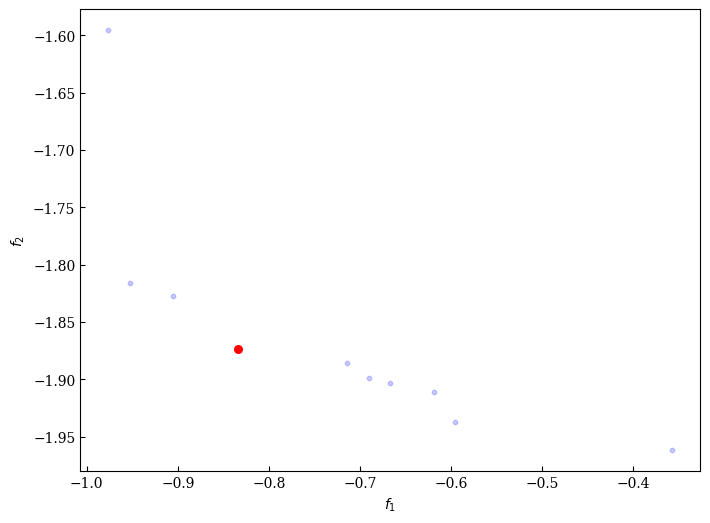
\includegraphics{TargetOptimization_files/figure-pdf/fig-pymoo-parks-output-1.png}

}

\subcaption{\label{fig-pymoo-parks-1}Multi-objective optimization Pareto
front. The selected solution is indicated in red.}

\end{minipage}%
%
\begin{minipage}{0.50\linewidth}

\centering{

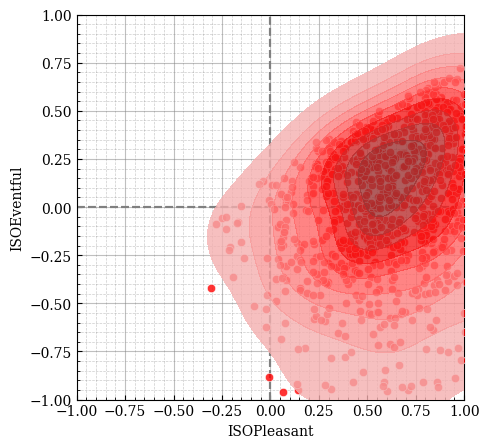
\includegraphics{TargetOptimization_files/figure-pdf/fig-pymoo-parks-output-2.png}

}

\subcaption{\label{fig-pymoo-parks-2}SCM distribution of the derived
target distribution.}

\end{minipage}%

\caption{\label{fig-pymoo-parks}NSGA-II optimization to learn the MSN
parameters which produce the Park ranking.}

\end{figure}%

\begin{Shaded}
\begin{Highlighting}[]
\BuiltInTok{print}\NormalTok{(park\_tgt.summary())}
\end{Highlighting}
\end{Shaded}

\begin{verbatim}
Fitted from direct parameters.
Direct Parameters:
xi:    [0.616 0.436]
omega: [[0.129 0.017]
 [0.017 0.296]]
alpha: [ 1.826 -7.109]


None
None
\end{verbatim}




\end{document}
